\documentclass{article}
\usepackage{amssymb}
\usepackage[dvips]{graphicx}
\usepackage{verbatim}
\usepackage{hyperref}
\usepackage{color}



\begin{document}

\title{SLS Detectors software installation}
\author{Anna Bergamaschi, Dhanya Thattil}
\date{\today}
\maketitle
\tableofcontents
\clearpage

%setcounter{tocdepth}{4} and \setcounter{secnumdepth}{4}







\section{The Software Package}
The SLS detectors software is intended to control the detectors developed by
the SLS Detectors group. The detectors currently supported are:

\indent MYTHEN, GOTTHARD, EIGER and JUNGFRAU.


The package provides software for the distributed system that comprises of
detectors, data receivers (to process detector data), and the client (to control
or monitor the system). The client and data receivers can be embedded in
the user's acquisitions system. Furthermore, the package also provides some
tools for detector calibration.

\subsection{Binaries}
\noindent The complete software package is composed of several programs which
can be installed (or locally compiled) depending on one's requirements:

\begin{itemize}

\item \textcolor{blue}{libSlsDetector.so, libSlsReceiver.so}:\\
The \textit{slsDetector shared and static libraries}, which are
necessary for all user interfaces. The \textit{C++ API} via the class
\textit{slsDetectorUsers} (installed with the default package) or the
\textit{Python API} via the class \textit{sls\_detector} (installed with the
package including Python API), which can be used from the user's acquisition
software to control the detectors and the data receivers.

\item \textcolor{blue}{sls\_detector\_put, sls\_detector\_get,
sls\_detector\_acquire, sls\_detector\_help}: \\
The \textit{command line interfaces}, which are provided to communicate with the
detectors and data receivers using the command line.

\item \textcolor{blue}{slsReceiver}: \\
The \textit{data receiver}, which can be run on a different machine than the
client, receives the data from the detector and processes it. The receiver can
be configured, controlled and monitored by the client.

\item \textcolor{blue}{slsMultiReceiver}: \\
It is the same as the \textit{slsReceiver}, but that it is a single process 
for many multiple slsReceiver child processes. One can configure the start TCP port,
number of slsReceiver processes and if call back should be enabled or not.

\item \textcolor{blue}{slsDetectorGUI}: \\
The \textit{graphical user interface}, which provides a user friendly way
of operating the detectors and data receivers with online data preview.

\item \textcolor{blue}{energyCalibrationWizard,angularCalibrationWizard}: \\
The \textit{calibration wizards} to analyze the data and produce the energy or
angular calibration files.

\item The \textit{virtual Detector servers} to simulate the detectors behavior.
However, only control commands work, not the data acquisition itself.
\end{itemize}




\section{Install Binaries via Conda}
This section is useful only if one wants to download only the binaries for
specific distribution and use the package via command line. Please refer later
sections to download source code and compile them.


One can download and install Miniconda via 

\url{https://conda.io/miniconda.html}


The conda package uses Travis CI for continuous integration with
automatic deployment to Anaconda Cloud. One can download only the package or the
package including the python interface.


After the installation, the binaries will be available in your path.

Please remember to clear shared memory after installation.
\begin{verbatim}
#displays list of shared memeory segments 
ipcs -m
#remove segments that have nattach equal to zero. They key is the first column
ipcrm -M [key]
\end{verbatim}

\begin{itemize}
 \item Only the package
\begin{verbatim}
#Add conda channels
conda config --add channels conda-forge
conda config --add channels slsdetectorgroup

#Install latest version
conda install sls_detector_lib
conda install sls_detector_gui

#Install specific release
conda install sls_detector_lib=4.0.0
conda install sls_detector_gui=4.0.0

\end{verbatim}
 \item The package including Python interface
\begin{verbatim}
#Add conda channels
conda config --add channels conda-forge
conda config --add channels sls_detector

#Install latest version
conda install sls_detector

#Install specific release 
conda install sls_detector=4.0.0

\end{verbatim}
\end{itemize}


\clearpage
\section{Install via Source Code}
This section is useful if one wants to use the API and embed it in their
acquisition system, or if one wants to download the source code and compile.

\subsection{Download Source Code}

\begin{itemize}
 \item Only the package
\begin{verbatim}
#Clone source code with specific release
git clone https://github.com/slsdetectorgroup/slsDetectorPackage.git --branch
4.0.0
\end{verbatim}
 \item The package including Python interface
\begin{verbatim}
#Clone source code with specific release
git clone https://github.com/slsdetectorgroup/sls_detector.git --branch
4.0.0
\end{verbatim}
\end{itemize}



\subsection{Requirements}
These are the basic requirements to install and use the software. Fine Tuning
the system will be discussed in other documentation provided.
\begin{itemize}

 \item \emph{C/C++}:\\
The software is written in C/C++. If Python API is used, it is a wrap around
to the C++ software.  Any Linux installation with working libgcc should be
sufficient.

 \item \emph{Shared Memory}:\\
Access to the shared memory of the control PC is required for the client.

 \item \emph{Network}:\\
The control PC communicates to the detectors and data receivers over TCP/IP.
Therefore, the detector should receive a proper IP address (either DHCP or
static) and no firewall should be present between the control PC and the
detector.

\item \emph{Compilation}:\\
cmake is required to compile. make is also possible, but is harder to find
dependencies.

\item \emph{GUI}:\\
To use the GUI, one requires atleast Qt4.8.2 and Qwt6.0. Installation of these
are discussed in the next sections.

\item \emph{Calibration Wizards}:\\
They are based on the CERN Root data analysis framework. Installation of it is
discussed in the next sections.

\end{itemize}


\subsubsection{Qt4 Installation for GUI}
It must be installed before Qwt. A Qt version equal or higher than 4.6 is
required. One can install it:
\begin{itemize}
 \item via YUM:
\begin{verbatim}
 yum install qt-devel
\end{verbatim}
 \item via download from:\\
\url{
https://download.qt.io/archive/qt/4.8/4.8.2/qt-everywhere-opensource-src-4.8.2.t
ar.gz} 


To install:
\begin{verbatim}
> gunzip qt-everywhere-opensource-src-4.8.2.tar.gz
> tar xvf qt-everywhere-opensource-src-4.8.2.tar
> ./configure
> make
> make install
\end{verbatim}
By default Qt4 will be installed in /usr/local/Trolltech/Qt-4.8.2/. 
\end{itemize}


\textbf{Setup Environment} 


One has to ensure that \verb=PATH= and \verb=LD_LIBRARY_PATH= have
been updated to include Qt4 install path, binaries and libraries.
Confirm by executing \verb=qmake -v= and ensuring the result points to Qt4 (not
Qt3 or Qt5). 


If the environment is not set up, one can add the libraries and
executables to the .bashrc by adding
\verb=LD_LIBRARY_PATH= and \verb=PATH=:
\begin{verbatim}
export QTDIR=/usr/local/Trolltech/Qt-4.8.2
export PATH=$QTDIR/bin:$PATH
export LD_LIBRARY_PATH=$QTDIR/lib:$LD_LIBRARY_PATH
\end{verbatim}


\subsubsection{Qwt Installation for GUI}
Before installing Qwt, one must install Qt
and ensure that \verb=QTDIR=, \verb=LD_LIBRARY_PATH= and \verb=PATH= point to
the correct Qt4
version.


A Qwt version equal or higher than 6 is required. One can
install it:
\begin{itemize}
 \item via YUM:
\begin{verbatim}
 yum install qwt-devel
\end{verbatim}
 \item via download from:\\
\url{
https://sourceforge.net/projects/qwt/files/qwt/6.0.0/qwt-6.0.0.zip/download}


To install:
\begin{verbatim}
> cd qwt-6.0.0
> qmake
> make
> make install
\end{verbatim}
By default Qwt will be installed int /usr/local/qwt-6.0.0 
\end{itemize}

\textbf{Setup Environment} 


One has to ensure that \verb=QWTDIR= and \verb=LD_LIBRARY_PATH= have
been updated to include Qwt install path and libraries.


If the environment is not set up, one can add the libraries to the
.bashrc by adding \verb=LD_LIBRARY_PATH=:
\begin{verbatim}
export QWTDIR=/usr/local/qwt-6.0.0/
export LD_LIBRARY_PATH=$QWTDIR/lib:$LD_LIBRARY_PATH
\end{verbatim}







\subsubsection{Root Installation for Calibration Wizards}
The software has been developed and tested with root 5.20, but any version
should work. One can download it from:
\begin{verbatim}
> svn co https://root.cern.ch/svn/root/trunk root
\end{verbatim}

\noindent To install:
\begin{verbatim}
> cd root
> ./configure --enable-qt
> make
> make install
\end{verbatim}

Edit your .bashrc to define the ROOTSYS enviroment variable and annd
the libraries and executables to the \verb=LD_LIBRARY_PATH= and \verb=PATH=:
\begin{verbatim}
export ROOTSYS=/usr/local/root-5.34
export PATH=$ROOTSYS/bin:$PATH
export LD_LIBRARY_PATH=$ROOTSYS/lib:$LD_LIBRARY_PATH
\end{verbatim}

You can also download the binaries, assuming that your linux and gcc versions
match as in:
\begin{verbatim}
http://root.cern.ch/drupal/content/production-version-534
\end{verbatim}





\subsection{Compilation}
One requires \verb=cmake= to compile and can be done in two ways:

\subsubsection{Using script cmk.sh}
The script uses \verb=cmake=. After compiling, the libraries and executables
will be found in `slsDetectorPackage/build/bin` directory.
Usage: [-c] [-b] [-h] [-d HDF5 directory] [-j]
\begin{itemize}
 \item -[no option]: only make
 \item -c: Clean
 \item -b: Builds/Rebuilds CMake files normal mode
 \item -h: Builds/Rebuilds Cmake files with HDF5 package
 \item -d: HDF5 Custom Directory
 \item -t: Build/Rebuilds only text client
 \item -r: Build/Rebuilds only receiver
 \item -g: Build/Rebuilds only gui
 \item -j: Number of threads to compile through
\end{itemize}

Some example options for compilation:

Most basic option: \verb=./cmk.sh -b=

For only make: \verb=./cmk.sh=

For make clean;make: \verb=./cmk.sh -c=

For using hdf5 without custom dir /blabla: \verb=./cmk.sh -h -d /blabla=

For rebuilding cmake without hdf5: \verb=./cmk.sh -b=

For using multiple cores to compile faster: \verb=./cmk.sh -j9=

For rebuilding only certain parts: \verb=./cmk.sh -tg= (only text client and
gui)


\subsubsection{Directly using cmake}

Use cmake to create out-of-source builds, by creating a build folder parallel to
source directory. 
\begin{verbatim}
 $ cd ..
 $ mkdir slsDetectorPackage-build
 $ cd slsDetectorPackage-build
 $ cmake ../slsDetectorPackage  -DCMAKE_BUILD_TYPE=Debug -DSLS_USE_HDF5=OFF 
 $ make
\end{verbatim}

Use the following as an example to compile statically and using specific hdf5
folder 
\begin{verbatim}
 $ HDF5_ROOT=/opt/hdf5v1.10.0 cmake ../slsDetectorPackage
-DCMAKE_BUILD_TYPE=Debug -DSLS_USE_HDF5=ON
\end{verbatim}

After compiling, the libraries and executables will be found at `bin` directory 
\begin{verbatim}
 $ ls bin/
    gui_client  libSlsDetector.a  libSlsDetector.so  libSlsReceiver.a 
libSlsReceiver.so    sls_detector_acquire  sls_detector_get  slsDetectorGui 
sls_detector_help sls_detector_put  slsReceiver
\end{verbatim}




\subsection{Setting environment variables}
One can set up the environment variables in the following ways.

\subsubsection{Using .bashrc file}
\begin{enumerate}
 \item \verb=emacs ~/.bashrc=
 \item Add the following function \verb=setup_slsdet= and replace \verb=path=
with absolute path of installed directory
\begin{verbatim}
function setup_slsdet
{ 
export PKGPATH=[path]
export LD_LIBRARY_PATH=$PKGPATH/slsDetectorPackage/build/bin:$LD_LIBRARY_PATH
export PATH=$PKGPATH/slsDetectorPackage/build/bin:$PATH
cd $PKGPATH/slsDetectorPackage/build/bin
} 
\end{verbatim}
  \item \verb=source ~/.bashrc=
  \item Next time, just run \verb=setup_slsdet= to load the environment
variables.
\end{enumerate}


One can also add the GUI environment variables if installed locally by adding
the following in the function \verb=setup_sldet= \\
\begin{verbatim}
export QTDIR=/path-where-it-is/Qt-4.8.2
export QWTDIR=/path-where-it-is/qwt-6.0.1
export QWT3D=/path-where-it-is/qwtplot3d
export QMAKESPEC=$QTDIR/mkspecs/linux-g++
export LD_LIBRARY_PATH=$QTDIR/lib:$QWTDIR/lib:$QWT3D/lib:$LD_LIBRARY _PATH
export PATH=$QTDIR/bin:$PATH
\end{verbatim}

\subsubsection{Without .bashrc file}
Go to binaries folder slsDetectorPackage/build/bin and execute the following:
\begin{verbatim}
export LD_LIBRARY_PATH=$PWD:$LD_LIBRARY_PATH
export PATH=$PWD:$PATH
\end{verbatim}


\subsection{Clean Shared Memory}
It is very crucial to clean the shared memory, before using a new version of
the SLS Detector Package or a different detector type.

One can use the \verb=cleansharedmemory.sh= script available under the
slsDetector Package.

One can also just delete the files that are typically located under /dev/shm/ folder
and starts with slsDetectorPackage.

One no longer has to delete segments using ipcs.


\section{Software Upgrade}

The upgrade of the package could require an upgrade of the on-board detector
server and/or firmware running on the detector as well.


\subsection{MYTHEN}
In such cases, the users are not expected to compile the software
themselves (which would require dedicated softwares) but only to download on the
detector board the programming files and/or software package provided by
the SLS Detectors group.

\subsubsection{MYTHEN Firmware}

To upgrade the firmware you need either a working version of the Altera
Quartus software or of the Quartus programmer, which can easily be downloaded
from: \\
\url{https://www.altera.com/download/programming/quartus2/pq2-index.jsp}
\medskip

\noindent Normally, installation of the software and of the driver for the
USB-Blaster (provided together with the MYTHEN detector) are simpler under
Windows. 


Under Windows, the first time that you connect the USB-Blaster to one
of your USB ports, you will be asked to install new hardware. Set the path to
search for the driver to:
\verb=C:\altera\80sp1\qprogrammer\drivers\usb-blasterp= (where 
\verb=C:\altera\80sp1\qprogrammer\= is assumed to be ther path where your
Quartus version is installed).
\begin{enumerate}
\item After starting the Quartus programmer, click on Hardware Setup and in the
"Currently selected hardware" window select USB-Blaster.
\item In the Mode combo box select "Active Serial Programming".
\item Plug the end of your USB-Blaster WITH THE ADAPTER PROVIDED in the
connector ASMI on the MCS board taking care that pin1 corresponds to the one
indexed and with the rectangualr pad.
\item Click on add file and from select the programming file provided when
the upgrade has been reccomended.
\item Check "Program/Configure" and "Verify".
\item Push the start button and wait until the programming process is
finished (progress bar top left).
\item In case the programmer gives you error messages, check the polarity of
your cable (pin1 corresponds) and that you have selected the correct programming
connector.
\end{enumerate}

\subsubsection{MYTHEN On-board Software}
\begin{enumerate}
 \item Connect to the board using telnet:
\begin{verbatim}
telnet  mymcs.mydomain.com
username: root
password: pass
\end{verbatim}
 \item Kill currently running servers and ensure \verb=/mnt/flash/root= exists.
\begin{verbatim}
killall mythenDetectorServer
ls /mnt/flash/root
#if the directory does not exist mkdir /mnt/flash/root
\end{verbatim}
 \item Transfer the provided software by ftp to the MCS.
\begin{verbatim}
ftp  mymcs.mydomain.com
username: root
password: pass
cd /mnt/flash/root
put mythenDetectorServer
quit
\end{verbatim}

\item After pressing reset on the board, the board should reboot.

\item If the program does not correctly start
 \begin{enumerate}
  \item Check by using the http interface that it is started by the inittab
(check that the file \verb=/mnt/etc/inittab= ends with the line \\
\verb=myid2:3:once:/mnt/flash/root/mythenDetectorServer=).  
  \item If program has not started, make the program executable by telnetting to
the MCS and executing: \\
\verb=chmod a+xrw  /mnt/flash/root/mythenDetectorServer=
  \item After pressing reset on the board, the board should reboot and the
acqusition program correctly start.
 \end{enumerate}
\end{enumerate}




\subsection{GOTTHARD}

In such cases, the users are not expected to compile the software
themselves (which would require dedicated softwares) but only to download on the
detector board the programming files and/or software package provided by
the SLS Detectors group.

\subsubsection{GOTTHARD Firmware}
\textit{For SLS Detector Package v4.0.0} \\
\indent Minimum compatible version: \\
\indent \indent 11.01.2013 \\
\indent Latest version:	\\
\indent \indent 08.02.2018 (50um) \\
\indent \indent 08.02.2018 (25 um Master) \\
\indent \indent 09.02.2018 (25 um Slave) \\

Normally, the firmware will be upgraded by us as it requires programming the
FPGA via the USB-Blaster.


To upgrade the firmware you need either a working version of the Altera
Quartus software or of the Quartus programmer, which can easily be downloaded
from: \\
\url{https://www.altera.com/download/programming/quartus2/pq2-index.jsp}


Normally, installation of the software and of the driver for the
USB-Blaster (provided together with the MYTHEN detector) are simpler under
Windows.


Under Windows, the first time that you connect the USB-Blaster to one
of your USB ports, you will be asked to install new hardware. Set the path to
search for the driver to:
\verb=C:\altera\80sp1\qprogrammer\drivers\usb-blasterp= (where 
\verb=C:\altera\80sp1\qprogrammer\= is assumed to be ther path where your
Quartus version is installed).
\begin{enumerate}
\item After starting the Quartus programmer, click on Hardware Setup and in the
"Currently selected hardware" window select USB-Blaster.
\item In the Mode combo box select "Active Serial Programming".
\item Plug the end of your USB-Blaster WITH THE ADAPTER PROVIDED in the
connector ASMI on the MCS board taking care that pin1 corresponds to the one
indexed and with the rectangualr pad.
\item Click on add file and from select the programming file provided when
the upgrade has been reccomended.
\item Check "Program/Configure" and "Verify".
\item Push the start button and wait until the programming process is
finished (progress bar top left).
\item In case the programmer gives you error messages, check the polarity of
your cable (pin1 corresponds) and that you have selected the correct programming
connector.
\end{enumerate}

\subsubsection{GOTTHARD On-board Software}
Every SLS Detector package release will have its coresponding matching on-board
server under \textbf{slsDetectorPackage/serverBin}.

\begin{enumerate}
  \item Install tftp if the pc does not have it.
  \item Copy the server from serverBin folder to /tftpboot (or equivalent tftp
folder) of the pc
  \item Copy the server to the detector by:
  \begin{enumerate}
    \item Connect to the blackfin on the detector\\ 
\verb=telnet bchipxxx=
    \item Prevent existing on-board server from respawning by:
    \begin{enumerate}
      \item Edit \verb=/etc/inittab= 
      \item Comment out the line
\verb=#ttyS0::respawn:/gotthardDetectorServervxxx= 
      \item Reboot blackfin using \verb=reboot=
      \item Run \verb=ps= to ensure no gotthardDetectorServers are running
    \end{enumerate}
    \item Copy new on-board server from pc to the blackfin using: \\
\verb=tftp pcxxx -r gotthardDetectorServerxxx -g= 
    \item Respawn the new server (server starts at detector statup): 
    \begin{enumerate}
      \item Edit \verb=/etc/inittab= 
      \item Uncomment out the line
\verb=ttyS0::respawn:/gotthardDetectorServervxxx= 
      \item Reboot blackfin using \verb=reboot=
      \item Run \verb=ps= to ensure that both the gotthardDetectorServers are
running.\\
\verb=gotthardDetectorServerxxx= \\
\verb=gotthardDetectorServerxxx 1953=
    \end{enumerate}
  \end{enumerate}
\end{enumerate}



\subsection{EIGER}

In such cases, the users are not expected to compile the software
themselves (which would require dedicated softwares) but only to download on the
detector board the programming files and/or software package provided by
the SLS Detectors group.

\subsubsection{EIGER Firmware}
\textit{For SLS Detector Package v4.0.0} \\
\indent Minimum compatible version:  22 \\
\indent Latest version:	22  \\


\begin{enumerate}
  \item One must get the latest package's corresponding bit files from the SLS
Detector Group.
  \item If one does not have the bcp script, that should also be obtained from
the SLS Detector Group. It is required to program the bit files and requires
that tftp be installed on the pc.
  \item Bring the detector into programmable mode by either of the following ways.
Both ways end up in just the central LED blinking.
  \begin{enumerate}
    \item hard reset on the back panel boards resulting in blinking LEDS 
    \item by having the following program running in the background. 
    \begin{verbatim}
    boot_recovery
    \end{verbatim}
\end{enumerate}
  \item Start a terminal for each half module and run the following to see 
progress.
\begin{verbatim}
	nc -p 3000 -u bebxxx 3000 
\end{verbatim}
  \item Run the following to update firmware
\begin{verbatim}
 #update back end fpga
bcp download.bit bebxxx:/fw0

 #update front left fpga
bcp download.bit bebxxx:/febl

 #update front right fpga
bcp download.bit bebxxx:/febr

 #update kernel
bcp download.bit bebxxx:/kernel
\end{verbatim}
Please update bit files with great caution as it could make your board
inaccessible, if done incorrectly.
\end{enumerate}



\subsubsection{EIGER On-board Software}
Every SLS Detector package release will have its coresponding matching on-board
server under \textbf{slsDetectorPackage/serverBin}.


Update the on-board software without connecting to the detector
\begin{verbatim}
#password for the boards: root

#Kill existing servers that are running on the detector
ssh root@beb031 killall eigerDetectorServer;

#Copy on-board server to detector inside executables folder
scp ~/path-where-it-is/eigerDetectorServerxxx root@bebxxx:~/executables;

#Overwrite the actual eigerDetectorServer on board
scp ~/path-where-it-is/eigerDetectorServerxxx
root@bebxxx:~/executables/eigerDetectorServer;

#sync
ssh root@bebxxx sync; 

#reboot the eiger board
\end{verbatim}


\bigskip One can connect to the detector by:
\begin{verbatim}
ssh root@bebxxx
password: root
\end{verbatim}


The on-board server is in ~/executables folder and respawned at startup in \\
\verb=/etc/rc5.d/S50board_com.sh= 





\subsection{JUNGFRAU}

In such cases, the users are not expected to compile the software
themselves (which would require dedicated softwares) but only to download on the
detector board the programming files and/or software package provided by
the SLS Detectors group.

\subsubsection{JUNGFRAU Firmware}
\textit{For SLS Detector Package v4.0.0} \\
\indent Minimum compatible version: 15.06.2018 \\
\indent Latest version: 15.06.2018 \\


At times, one has to update the firmware, which then also requires updating the
on-board software. 


\textbf{\textit{Jungfrau firmware can be upgraded via the SLS Detector Package
binaries from the command line.}}

\begin{enumerate}
  \item One must get the latest package's corresponding POF file from the SLS
Detector Group.
  \item Update the latest SLS Detector package installed.
  \item Update the on-board software as per the instructions in the next
section.
  \item Start the on-board server in update mode:
  \begin{enumerate}
    \item Connect to the blackfin on the detector\\ 
\verb=telnet bchipxxx=
    \item Prevent existing on-board server from respawning by:
    \begin{enumerate}
      \item Edit \verb=/etc/inittab= 
      \item Comment out the line
\verb=#ttyS0::respawn:/jungfrauDetectorServervxxx= 
      \item Reboot blackfin using \verb=reboot=
      \item Run \verb=ps= to ensure no jungfrauDetectorServers are running
    \end{enumerate}
    \item Start the server in update mode using: \\
\verb=./jungfrauDetectorServerxxx -update= \\
    Leave this console on to come back to it later.
  \end{enumerate}
  \item From the command line of the pc, clear shared memory \\
\verb=./sls_detector_get free= \\
  If one gets shmget error, please clean the shared memory properly using the
script in \verb=slsDetectorPackage/cleansharedmemory.sh=
  \item Add the detector to shared memory using \\
\verb=./sls_detector_put hostname bchipxxx=
  \item Program the FPGA using \\
\verb=./sls_detector_put programfpga xxx.pof= 
  \item Once the programming is done:
  \begin{enumerate}
    \item Switch to the console that has the update server running and kill it
using Ctrl+C and ensure no jungfrauDetectorServers are
running
    \item Restart the new server to see if it runs with the new firmware \\
\verb=./jungfrauDetectorServerxxx= \\
If the server didn't start properly, please contact us with the error message
shown when starting the server up, else continue with the following steps.
    \item Respawn the new server (server starts at detector statup): 
    \begin{enumerate}
      \item Edit \verb=/etc/inittab= 
      \item Uncomment out the line
\verb=ttyS0::respawn:/jungfrauDetectorServervxxx= 
      \item Reboot blackfin using \verb=reboot=
      \item Run \verb=ps= to ensure that both the gotthardDetectorServers are
running.\\
\verb=jungfrauDetectorServervxxx= \\
\verb=jungfrauDetectorServervxxx 1953=
    \end{enumerate}
  \end{enumerate}

\end{enumerate}



\subsubsection{JUNGFRAU On-board Software}
Every SLS Detector package release will have its coresponding matching on-board
server under \textbf{slsDetectorPackage/serverBin}.


\begin{enumerate}
  \item Install tftp if the pc does not have it.
  \item Copy the server from serverBin folder to /tftpboot (or equivalent tftp
folder) of the pc
  \item Copy the server to the detector by:
  \begin{enumerate}
    \item Connect to the blackfin on the detector\\ 
\verb=telnet bchipxxx=
    \item Prevent existing on-board server from respawning by:
    \begin{enumerate}
      \item Edit \verb=/etc/inittab= 
      \item Comment out the line
\verb=#ttyS0::respawn:/jungfrauDetectorServervxxx= 
      \item Reboot blackfin using \verb=reboot=
      \item Run \verb=ps= to ensure no gotthardDetectorServers are running
    \end{enumerate}
    \item Copy new on-board server from pc to the blackfin using: \\
\verb=tftp pcxxx -r jungfrauDetectorServervxxx -g= 
    \item Respawn the new server (server starts at detector statup): 
    \begin{enumerate}
      \item Edit \verb=/etc/inittab= 
      \item Uncomment out the line
\verb=ttyS0::respawn:/jungfrauDetectorServervxxx= 
      \item Reboot blackfin using \verb=reboot=
      \item Run \verb=ps= to ensure that both the gotthardDetectorServers are
running.\\
\verb=jungfrauDetectorServervxxx= \\
\verb=jungfrauDetectorServervxxx 1953=
    \end{enumerate}
  \end{enumerate}
\end{enumerate}






\begin{comment}
\section{Detector system architecture}

For most users the detector will be composed by a single module. Therefore all configurations of the detector will refere to that single entity.

However, for some experiments it is necessary to concatenate the data from several detector controllers, and sometimes (e.g. MYTHEN) each controller can control many modules. This should be transparent to the user since most parameters will be identical for all controllers (e.g. exposure time, energy threshold etc.), except for the configurations specific to the controller (e.g. hardware configuration).\\
In principle it is possible to combine controllers of different type (e.g. MYTHEN, GOTTHARD, EIGER) but the user should then evaluate if it really makes sense to control such different systems in parallel.

In other cases, several SLS detectors will independently acquire data during the same experiment. In this case it will be necessary to be able to seperately control them.

The detectors can be controlled in parallel from several PCs (clients). However it is important the the configurations match on all of the them such that no conflict arise. Eventually a detector can be locked to a specific control PC, still different users interfaces (command line, GUI) can be used in parallel.

A sketch of a possible complex detector configuration is shown in figure~\ref{fig:multi_detector}
\subsection{Detector indexes}
For this reason and index is assigned to each detector. If a single detector is used, as in most cases, the index will be omitted and defaults to 0.\\
To control the other detectors the index cannot be omitted!\\


An index will also be assigned to each controller within a detector. However the user normally will not need to address single controllers, except for the most advanced settings which can be left to configuration files.\\


Finally each module within a controller has an internal index. However in general it is not required that the user is aware of the system architecture and, if needed (rarely), the modules can simply be addressed sequentially starting from controller 0.



\begin{figure}
\caption{Scketch of a possible complex system architecture composed of several detector, each consisting in many controllers eventually controlling several modules.}\label{fig:multidet}
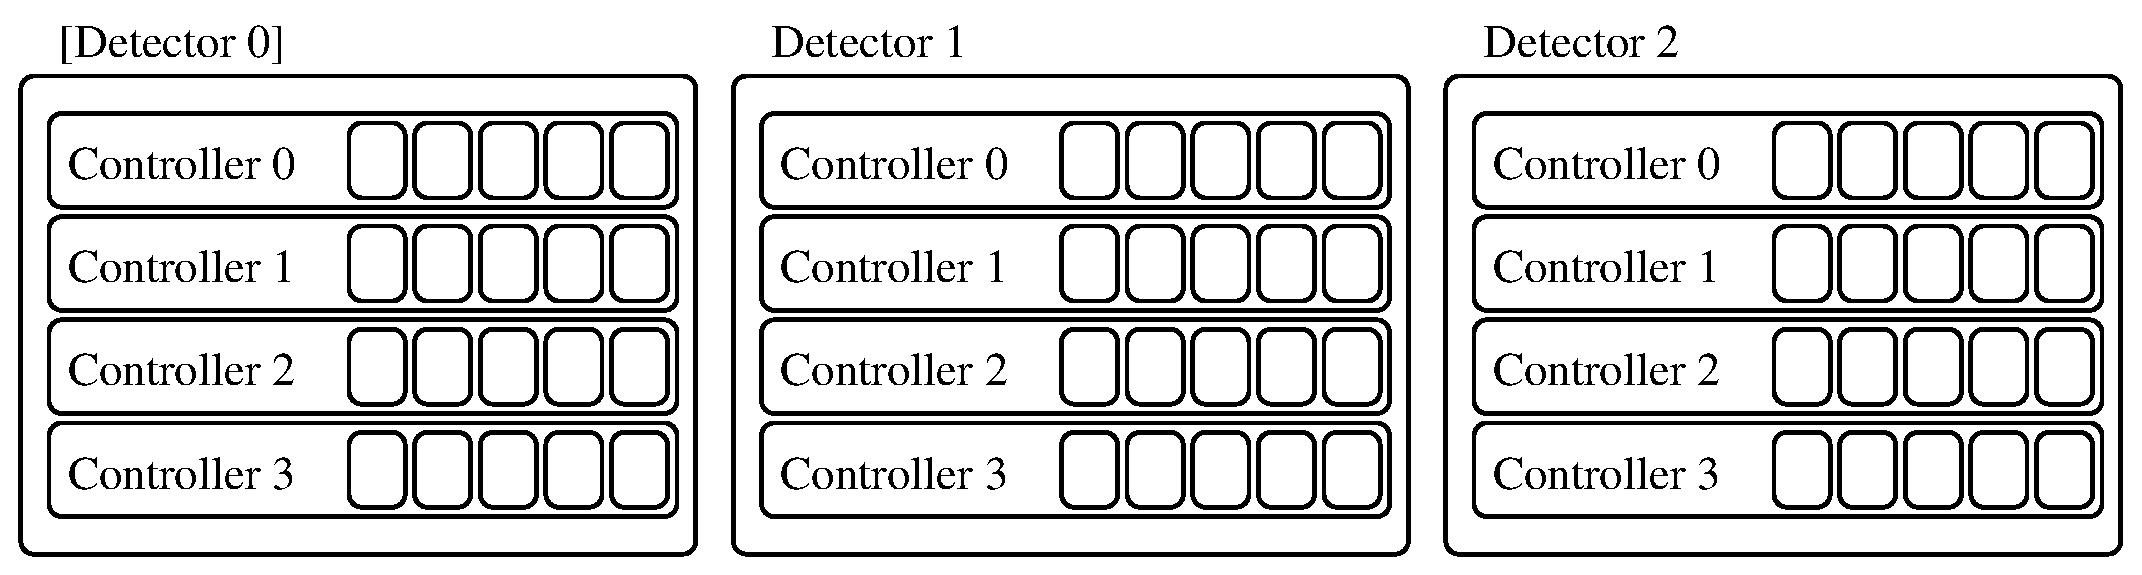
\includegraphics[width=\textwidth]{multi_detector}
\end{figure} 

\subsection{Data receiver}

For slower acquisitions, the detector will return the data to the control PC over TCP/IP (e.g. MYTHEN).

However, for faster frame rates (e.g. GOTTHARD, EIGER) the controllers will return the data to a data receiver i.e. a process specifically designed to receive the data from the controller over a GBit network and save them to disk. \\
The data receiver can run on any machine (e.g. a file server) accessible by both the control PC and the detector controller, as sketched in figure~\ref{fig:datareceiver}.

After starting the data receiver process and correctly configuring the client and the detector, this architecture should be completely transparent for the user, except that the output file path must be properly configured from the client for the data receiver machine (easiest is that the disk is mounted for both machines in the same location).\\
The cleint will take care of communicating with the data receiver and the detector. A feedback about the progress of the acquisition and a preview of the data being acquired can also be obtained by the client from the data receiver.


\begin{figure}
\caption{Scketch of the comminication between the control PC, the detector and the data receiver.}\label{fig:datareceiver}
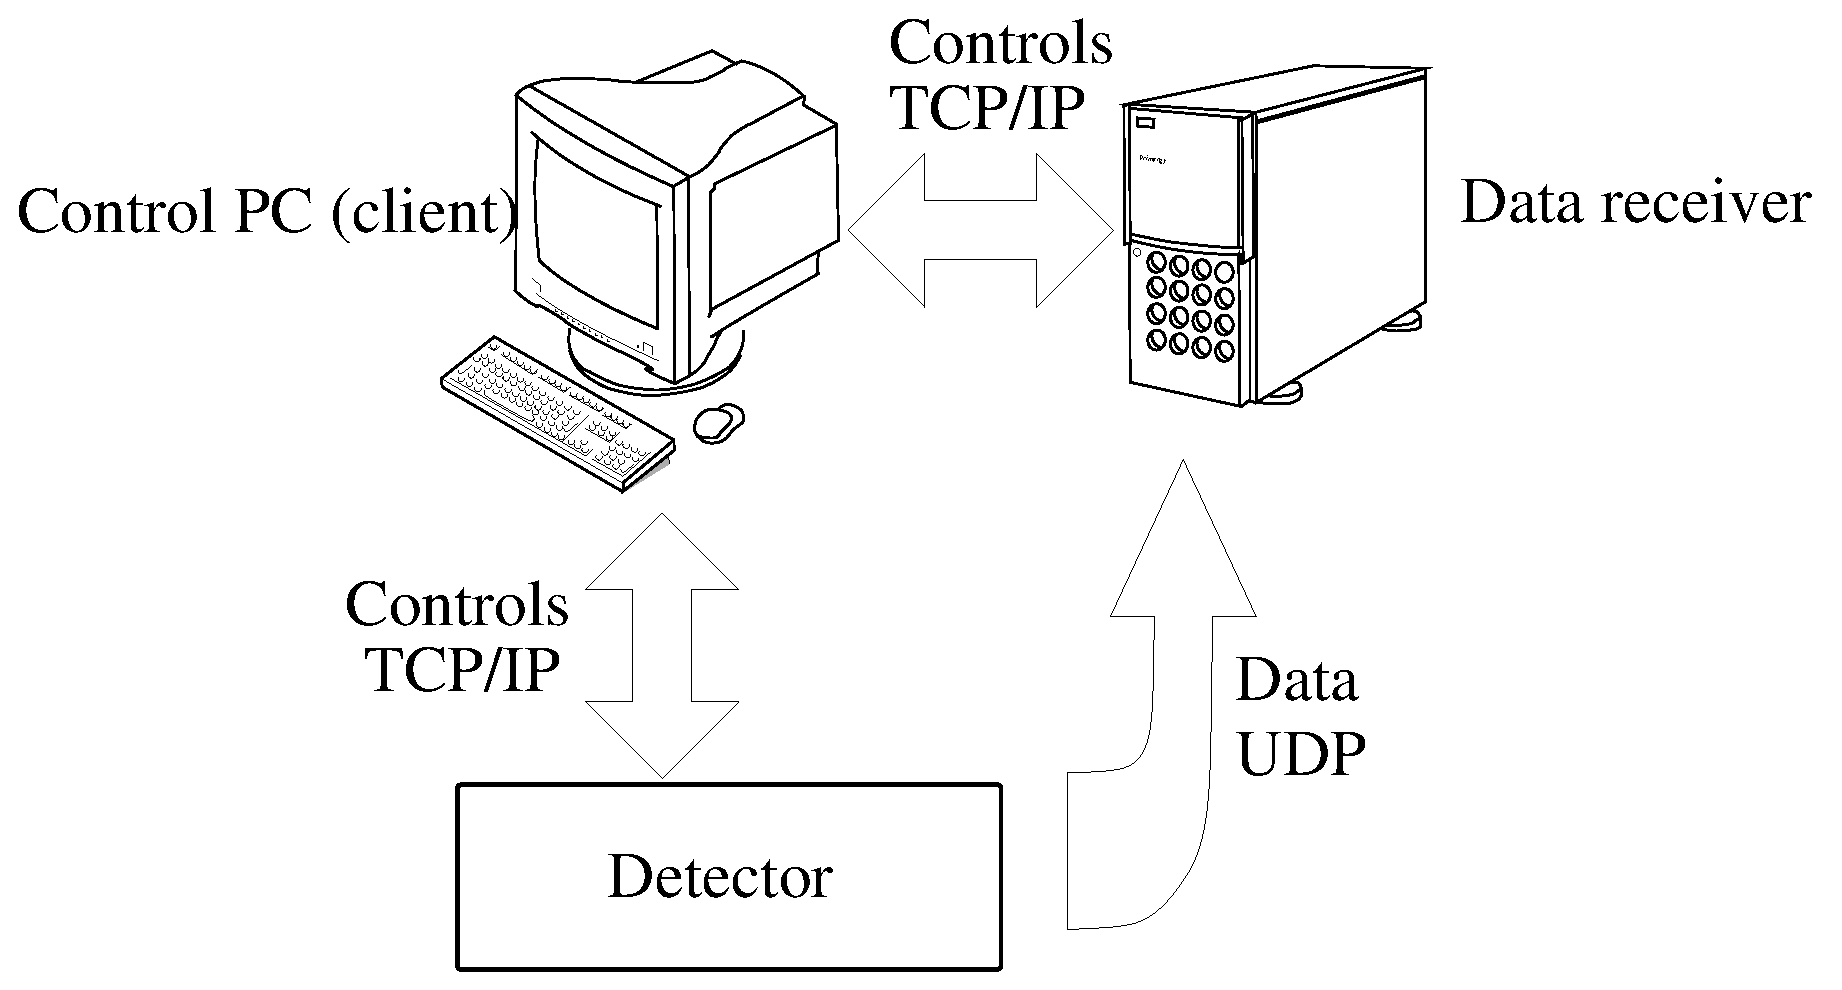
\includegraphics[width=\textwidth]{data_receiver}
\end{figure} 

\subsection{Examples}

For MYTHEN, if one needs to control 6 modules, the system can either be composed by and MCS6 with 6 modules (1 detector, 1 controller, 6 modules), or by 6 MCS1 (1 detector, 6 controller, 1 module each). After apppropriate configuration of the system, the interface to the user will be the same for both systems.

For GOTTHARD, one module corresponds to one controller. A detector will have the smae number of controllers and modules.

For EIGER, one module consists in two controllers. Fo a multi-module system, the number of controllers will increase accordingly, but should be left to a configuration file.

You will need to configure more than one detector, only in case you want to operate several detectors independently.


\section{The trimbits and calibration files} \label{sec:trimdir}


\subsection{MYTHEN}
In order to be able to properly operate your detector you need a directory where the trimbit files (needed to set the detector settings and eventually equalize the individual channel thresholds) which in the following will be named \textit{settingsdir} and a directory where the calibration files (needed to convert the threshold energy in DAC units) are stored which in the following will be named \textit{caldir}. \\
\textit{settingsdir} and \textit{caldir} can even be the same directory, and an example of it is given in the software package by the example directory \verb=trimdir=. 
Since these directories are customized by producing trimbit files and calibration for each detector, make sure not to overwrite yours every time you upgrade the software.

\textit{settingsdir} should contain three subdirectories \verb=standard=,  \verb=fast= and  \verb=highgain= containing respectively the trimfiles \verb=standard.trim=,  \verb=fast.trim= and  \verb=highgain.trim= which contain the correct voltage settings for the detector although all the individual channel thresholds set to 0. The original files contained in the package should be used, infact in case of error the detector would not recognize the correct settings.\\
The default trimbit files for each file will be stored in the directory according to the settings with the name \verb=noise.snxxx= where \verb=xxx= is the module serial number.\\

\textit{caldir} should contain three subdirectories \verb=standard=,  \verb=fast= and  \verb=highgain= containing respectively the trimfiles \verb=standard.cal=,  \verb=fast.cal= and  \verb=highgain.cal= which contain an average calibration of the modules for the diffrent settings. However this can different from the correct one for each individual module even of several kev and therefore it is very important to perform an energy calibration on a module basis.\\
The default calibration files for each file will be stored in the directory according to the settings with the name \verb=calibration.snxxx= where \verb=xxx= is the module serial number.

The \textit{settingsdir} and \textit{caldir} should be properly configured for your detector either in a configuration file (for use with text clients, GUI or API) or dynamically (works only for the text clients).

\subsection{GOTTHARD}
A \textit{settingsdir} should be configured, as the directory  \verb=settings= in this software package.\\
It must contain the subdirectories \verb=dynamicgain=, \verb=gain1=, 
\verb=gain2=,  \verb=gain3=,  \verb=highgain=,  \verb=lowgain=, 
\verb=mediumgain=, and   \verb=veryhighgain= in order to properly configure the
GOTTHARD detector using the various gain settings.

\end{comment}

\end{document}

